\documentclass[mstat,12pt]{unswthesis}

\usepackage{color}
\usepackage{fancyvrb}
\newcommand{\VerbBar}{|}
\newcommand{\VERB}{\Verb[commandchars=\\\{\}]}
\DefineVerbatimEnvironment{Highlighting}{Verbatim}{commandchars=\\\{\}}
% Add ',fontsize=\small' for more characters per line
\usepackage{framed}
\definecolor{shadecolor}{RGB}{248,248,248}
\newenvironment{Shaded}{\begin{snugshade}}{\end{snugshade}}
\newcommand{\AlertTok}[1]{\textcolor[rgb]{0.94,0.16,0.16}{#1}}
\newcommand{\AnnotationTok}[1]{\textcolor[rgb]{0.56,0.35,0.01}{\textbf{\textit{#1}}}}
\newcommand{\AttributeTok}[1]{\textcolor[rgb]{0.77,0.63,0.00}{#1}}
\newcommand{\BaseNTok}[1]{\textcolor[rgb]{0.00,0.00,0.81}{#1}}
\newcommand{\BuiltInTok}[1]{#1}
\newcommand{\CharTok}[1]{\textcolor[rgb]{0.31,0.60,0.02}{#1}}
\newcommand{\CommentTok}[1]{\textcolor[rgb]{0.56,0.35,0.01}{\textit{#1}}}
\newcommand{\CommentVarTok}[1]{\textcolor[rgb]{0.56,0.35,0.01}{\textbf{\textit{#1}}}}
\newcommand{\ConstantTok}[1]{\textcolor[rgb]{0.00,0.00,0.00}{#1}}
\newcommand{\ControlFlowTok}[1]{\textcolor[rgb]{0.13,0.29,0.53}{\textbf{#1}}}
\newcommand{\DataTypeTok}[1]{\textcolor[rgb]{0.13,0.29,0.53}{#1}}
\newcommand{\DecValTok}[1]{\textcolor[rgb]{0.00,0.00,0.81}{#1}}
\newcommand{\DocumentationTok}[1]{\textcolor[rgb]{0.56,0.35,0.01}{\textbf{\textit{#1}}}}
\newcommand{\ErrorTok}[1]{\textcolor[rgb]{0.64,0.00,0.00}{\textbf{#1}}}
\newcommand{\ExtensionTok}[1]{#1}
\newcommand{\FloatTok}[1]{\textcolor[rgb]{0.00,0.00,0.81}{#1}}
\newcommand{\FunctionTok}[1]{\textcolor[rgb]{0.00,0.00,0.00}{#1}}
\newcommand{\ImportTok}[1]{#1}
\newcommand{\InformationTok}[1]{\textcolor[rgb]{0.56,0.35,0.01}{\textbf{\textit{#1}}}}
\newcommand{\KeywordTok}[1]{\textcolor[rgb]{0.13,0.29,0.53}{\textbf{#1}}}
\newcommand{\NormalTok}[1]{#1}
\newcommand{\OperatorTok}[1]{\textcolor[rgb]{0.81,0.36,0.00}{\textbf{#1}}}
\newcommand{\OtherTok}[1]{\textcolor[rgb]{0.56,0.35,0.01}{#1}}
\newcommand{\PreprocessorTok}[1]{\textcolor[rgb]{0.56,0.35,0.01}{\textit{#1}}}
\newcommand{\RegionMarkerTok}[1]{#1}
\newcommand{\SpecialCharTok}[1]{\textcolor[rgb]{0.00,0.00,0.00}{#1}}
\newcommand{\SpecialStringTok}[1]{\textcolor[rgb]{0.31,0.60,0.02}{#1}}
\newcommand{\StringTok}[1]{\textcolor[rgb]{0.31,0.60,0.02}{#1}}
\newcommand{\VariableTok}[1]{\textcolor[rgb]{0.00,0.00,0.00}{#1}}
\newcommand{\VerbatimStringTok}[1]{\textcolor[rgb]{0.31,0.60,0.02}{#1}}
\newcommand{\WarningTok}[1]{\textcolor[rgb]{0.56,0.35,0.01}{\textbf{\textit{#1}}}}


%%%%%%%%%%%%%%%%%%%%%%%%%%%%%%%%%%%%%%%%%%%%%%%%%%%%%%%%%%%%%%%%%%
% 
% OK...Now we get to some actual input.  The first part sets up
% the title etc that will appear on the front page
%
%%%%%%%%%%%%%%%%%%%%%%%%%%%%%%%%%%%%%%%%%%%%%%%%%%%%%%%%%%%%%%%%%

\title{Rapport de groupe en Sciences des Données 2 et Bases de données}

\authornameonly{Katia Djellali (22113493), Elise
Commandré(22104606), Alvin Ingabire(22111286), Cédric Henry(22105033). }

\author{\Authornameonly}

\copyrightfalse
\figurespagefalse
\tablespagefalse

%%%%%%%%%%%%%%%%%%%%%%%%%%%%%%%%%%%%%%%%%%%%%%%%%%%%%%%%%%%%%%%%%
%
%  And now the document begins
%  The \beforepreface and \afterpreface commands puts the
%  contents page etc in
%
%%%%%%%%%%%%%%%%%%%%%%%%%%%%%%%%%%%%%%%%%%%%%%%%%%%%%%%%%%%%%%%%%%


\linespread{1}
\usepackage{amsfonts}
\usepackage{amssymb}
\usepackage{amsthm}
\usepackage{latexsym,amsmath}
\usepackage{graphicx}
\usepackage{afterpage}
\usepackage[colorlinks]{hyperref}
 \hypersetup{
     colorlinks=true,
     linkcolor=black,
     filecolor=black,
     citecolor= black,      
     urlcolor=cyan,
     }
\usepackage{textcomp}
\usepackage{longtable}
\usepackage{booktabs}
\usepackage{float}
\let\origfigure\figure
\let\endorigfigure\endfigure
\renewenvironment{figure}[1][2] {
    \expandafter\origfigure\expandafter[H]
} {
    \endorigfigure
}
\usepackage[T1]{fontenc}
\usepackage{ragged2e}
\def\tightlist{}


\newcommand{\R}{\mathbb{R}}
\newcommand{\Q}{\mathbb{Q}}
\newcommand{\C}{\mathbb{C}}
\newcommand{\N}{\mathbb{N}}
\newcommand{\F}{\mathbb{F}}
\newcommand{\PP}{\mathbb{P}}
\newcommand{\T}{\mathbb{T}}
\newcommand{\Z}{\mathbb{Z}}
\newcommand{\B}{\mathfrak{B}}
\newcommand{\BB}{\mathcal{B}}
\newcommand{\M}{\mathfrak{M}}
\newcommand{\X}{\mathfrak{X}}
\newcommand{\Y}{\mathfrak{Y}}
\newcommand{\CC}{\mathcal{C}}
\newcommand{\E}{\mathbb{E}}
\newcommand{\cP}{\mathcal{P}}
\newcommand{\cS}{\mathcal{S}}
\newcommand{\A}{\mathcal{A}}
\newcommand{\ZZ}{\mathcal{Z}}

\newcommand{\bv}[1]{\mbox{BV($#1$)}}
\newcommand{\comb}[2]{\left(\!\!\!\begin{array}{c}#1\\#2\end{array}\!\!\!\right)
}
\newcommand{\Lat}{{\rm Lat}}
\newcommand{\var}{\mathop{\rm var}}
\newcommand{\Pt}{{\mathcal P}}
\def\tr(#1){{\rm trace}(#1)}
\def\Exp(#1){{\mathbb E}(#1)}
\def\Exps(#1){{\mathbb E}\sparen(#1)}
\newcommand{\floor}[1]{\left\lfloor #1 \right\rfloor}
\newcommand{\ceil}[1]{\left\lceil #1 \right\rceil}
\newcommand{\hatt}[1]{\widehat #1}
\newcommand{\modeq}[3]{#1 \equiv #2 \,(\text{mod}\, #3)}
\newcommand{\rmod}{\,\mathrm{mod}\,}
\newcommand{\p}{\hphantom{+}}
\newcommand{\vect}[1]{\mbox{\boldmath $ #1 $}}
\newcommand{\reff}[2]{\ref{#1}.\ref{#2}}
\newcommand{\psum}[2]{\sum_{#1}^{#2}\!\!\!'\,\,}
\newcommand{\bin}[2]{\left( \begin{array}{@{}c@{}}
				#1 \\ #2
			\end{array}\right)	}


\newcommand{\be}{($\beta$)}
\newcommand{\eqp}{\mathrel{{=}_p}}
\newcommand{\ltp}{\mathrel{{\prec}_p}}
\newcommand{\lep}{\mathrel{{\preceq}_p}}
\def\brack#1{\left \{ #1 \right \}}
\def\bul{$\bullet$\ }
\def\cl{{\rm cl}}
\let\del=\partial
\def\enditem{\par\smallskip\noindent}
\def\implies{\Rightarrow}
\def\inpr#1,#2{\t \hbox{\langle #1 , #2 \rangle} \t}
\def\ip<#1,#2>{\langle #1,#2 \rangle}
\def\lp{\ell^p}
\def\maxb#1{\max \brack{#1}}
\def\minb#1{\min \brack{#1}}
\def\mod#1{\left \vert #1 \right \vert}
\def\norm#1{\left \Vert #1 \right \Vert}
\def\paren(#1){\left( #1 \right)}
\def\qed{\hfill \hbox{$\Box$} \smallskip}
\def\sbrack#1{\Bigl \{ #1 \Bigr \} }
\def\ssbrack#1{ \{ #1 \} }
\def\smod#1{\Bigl \vert #1 \Bigr \vert}
\def\smmod#1{\bigl \vert #1 \bigr \vert}
\def\ssmod#1{\vert #1 \vert}
\def\sspmod#1{\vert\, #1 \, \vert}
\def\snorm#1{\Bigl \Vert #1 \Bigr \Vert}
\def\ssnorm#1{\Vert #1 \Vert}
\def\sparen(#1){\Bigl ( #1 \Bigr )}

\newcommand\blankpage{%
    \null
    \thispagestyle{empty}%
    \addtocounter{page}{-1}%
    \newpage}



\newtheorem{theorem}{Theorem}[section]
\newtheorem{lemma}[theorem]{Lemma}
\newtheorem{proposition}[theorem]{Proposition}
\newtheorem{corollary}[theorem]{Corollary}
\newtheorem{conjecture}[theorem]{Conjecture}
\newtheorem{definition}[theorem]{Definition}
\newtheorem{example}[theorem]{Example}
\newtheorem{remark}[theorem]{Remark}
\newtheorem{question}[theorem]{Question}
\newtheorem{notation}[theorem]{Notation}
\numberwithin{equation}{section}



\hyphenation{Mar-cin-kie-wicz Rade-macher}


\newlength{\cslhangindent}
\setlength{\cslhangindent}{1.5em}
\newlength{\csllabelwidth}
\setlength{\csllabelwidth}{1.5em}
\newenvironment{CSLReferences}[2] % #1 hanging-ident, #2 entry spacing
 {% don't indent paragraphs
  \setlength{\parindent}{0pt}
  % turn on hanging indent if param 1 is 1
  \ifodd #1 \everypar{\setlength{\hangindent}{\cslhangindent}}\ignorespaces\fi
  % set entry spacing
  \ifnum #2 > 0
  \setlength{\parskip}{#2\baselineskip}
  \fi
 }%
 {}
\usepackage{calc} % for \widthof, \maxof
\newcommand{\CSLBlock}[1]{#1\hfill\break}
\newcommand{\CSLLeftMargin}[1]{\parbox[t]{\maxof{\widthof{#1}}{\csllabelwidth}}{#1}}
\newcommand{\CSLRightInline}[1]{\parbox[t]{\linewidth}{#1}}
\newcommand{\CSLIndent}[1]{\hspace{\cslhangindent}#1}






\renewcommand{\contentsname}{Table des matières}

\renewcommand{\chaptername}{Chapitre}



\begin{document}

\beforepreface

%\afterpage{\blankpage}

% plagiarism

\prefacesection{Déclaration de non plagiat}

\vskip 2pc \noindent Nous déclarons que ce rapport est le fruit de notre seul travail, à part lorsque cela est indiqué  explicitement. 

\vskip 2pc  \noindent Nous acceptons que la personne évaluant ce rapport puisse, pour les besoins de cette évaluation:
\begin{itemize}
\item la reproduire et en fournir une copie à un autre membre de l'université; et/ou,
\item en communiquer une copie à un service en ligne de détection de plagiat (qui pourra en retenir une copie pour les besoins d'évaluation future).
\end{itemize}

\vskip 2pc \noindent Nous certifions que nous avons lu et compris les règles ci-dessus.\vspace{24pt}

\vskip 2pc \noindent En signant cette déclaration, nous acceptons ce qui précède.
\vskip 2pc \noindent
Signature: Commandré Elise \rule{7cm}{0.25pt} \hfill Date: 05/05/2023 \rule{4cm}{0.25pt} \\[1cm]
Signature: Djellali Katia\rule{7cm}{0.25pt} \hfill Date: 05/05/2023 \rule{4cm}{0.25pt} \\[1cm]
Signature: Ingabire Alvin\rule{7cm}{0.25pt} \hfill Date: 05/05/2023\rule{4cm}{0.25pt} \\[1cm]
Signature: Henry Cédric\rule{7cm}{0.25pt} \hfill Date: 05/05/2023\rule{4cm}{0.25pt} \\[1cm]
\vskip 1pc

%\afterpage{\blankpage}


% Abstract


\afterpreface





%%%%%%%%%%%%%%%%%%%%%%%%%%%%%%%%%%%%%%%%%%%%%%%%%%%%%%%%%%%%%%%%%%
%
% Now we can start on the first chapter
% Within chapters we have sections, subsections and so forth
%
%%%%%%%%%%%%%%%%%%%%%%%%%%%%%%%%%%%%%%%%%%%%%%%%%%%%%%%%%%%%%%%%%%



%%%%%%%%%%%%%%%%%%%%%%%%%%%%%%%%%%%%%

%\afterpage{\blankpage}


\hypertarget{introduction}{%
\chapter{Introduction}\label{introduction}}

Pour le projet, nous avons choisi le sujet suivant: ``Où mange-t-on le
mieux?''. Nous nous sommes longtemps interrogés sur comment interpréter
ce sujet qui pouvait rapidement devenir assez vaste : devions-nous
travailler en fonction du type de restauration (restaurants scolaires,
restaurants gastronomiques, etc.), c'est-à-dire en les comparant ou
devions-nous plus nous concentrer sur les grandes villes et non les
petits villages\ldots{} Nous en sommes arrivés à la conclusion de nous
concentrer sur les restaurants dans les grandes villes et de ne prendre
en compte que les restaurants ayant des notes (étoles, avis, notes
sanitaires, etc.) . En approfondissant ainsi les recherches, nous nous
sommes tournés vers la problématique :

\bigskip

\centering

\textbf{Où mange-t-on le mieux dans les grandes villes?}

\bigskip

\hypertarget{donnuxe9es}{%
\chapter{Données}\label{donnuxe9es}}

\hypertarget{pruxe9sentation-des-donnuxe9es}{%
\section{Présentation des
données}\label{pruxe9sentation-des-donnuxe9es}}

\justifying

Pour répondre à cette problématique, nous avons décidé d'utiliser le jeu
de données fourni par les enseignants issu de data.gouv.fr ainsi qu'un
autre jeu de données trouvé en ligne sur le site Kaggle:

\begin{itemize}
\item
  Jeu de données 1 ( 12 colonnes et 34 013 lignes) :
  ``export\_alimconfiance.xls'' fourni par nos enseignants suivant le
  thème choisi. Il répertorie différents établissements situés en France
  dans lesquels on a procédé à une inspection sanitaire. Source :
  \url{https://www.data.gouv.fr/fr/datasets/resultats-des-controles-officiels-sanitaires-dispositif-dinformation-alimconfiance/}
\item
  Jeu de données 2 (12 colonnes et 6 781 lignes) : Il répertorie les
  restaurants étoilés au guide Michelin dans le monde. Source :
  \url{https://www.kaggle.com/datasets/ngshiheng/michelin-guide-restaurants-2021}.
\end{itemize}

\hypertarget{nettoyage-des-donnuxe9es}{%
\section{Nettoyage des données}\label{nettoyage-des-donnuxe9es}}

Les données utilisées étaient très volumineuses et avaient des
propriétés (colonnes) qui n'avaient aucune pertinence, ce qui nous
aurait ralenti au moment de faire des requêtes. Nous avons donc supprimé
les colonnes et lignes non pertinentes et sur certaines colonnes et
lignes nous avons choisi de filtrer quelques éléments pour ne garder que
ceux qui nous intéresse.

\begin{itemize}
\item
  Jeu de données 1: Pour ce jeu de données, on ne va s'intéresser qu'aux
  restaurants ; on a donc filtré la colonne libéllé pour ne garder que
  les restaurants et on supprimé les colonnes ``ods\_type\_activité'' et
  ``Agrement'' qui ne donnaient aucune information supplémentaire.
  ``Agrement'' n'avait pas de valeur pour la plupart des établissements.
  On a ainsi obtenu un jeux de données avec 11 658 lignes et 7 colonnes
  comme le nom du restaurant, son adresse, le code postal et sa commune,
  l'avis de l'évaluation sanitaire, et les coordonnées du restaurant.
  Les notes d'hygiènes étant caractérisées par des adjectifs allant de
  satisfaisant à très satisfaisant, nous avons modifié la colonne en
  remplaçant ces adjectifs par des chiffres allant de un à trois afin de
  faciliter les calculs de nos futures requêtes : très satisfaisant = 3,
  satisfaisant = 2 et à améliorer = 1.
\item
  Jeu de données 2: On a filtré les données pour ne garder que les
  restaurants situés en France (en filtrant la colonne « Location » ) et
  on a supprimé les colonnes ne nous intéressant pas telles que «
  Facilities and Services » car non pertinentes pour les requêtes. On
  obtient alors un nouveau jeu de données composé de 10 colonnes et 242
  lignes : il est composé du nom du restaurant, de son adresse, du nom
  de la ville, du prix (échelle de prix), du type de cuisine, de sa
  longitude et latitude, de son numéro de téléphone, de son site web et
  du nombre d'étoiles. L'échelle de prix étant illustré par un nombre de
  symboles « € », nous avons modifié la colonne en remplaçant le nombre
  de symbole par les chiffres correspondant (de un à trois) afin de
  faciliter les calculs de nos futures requêtes.
\end{itemize}

\hypertarget{descriptif-des-jeux-de-donnuxe9es}{%
\section{Descriptif des jeux de
données}\label{descriptif-des-jeux-de-donnuxe9es}}

\begin{longtable}[]{@{}ccc@{}}
\toprule()
Nom colonne & Type & Signification \\
\midrule()
\endhead
App\_libelle\_etablissement & Varchar & Nom du restaurant \\
Adresse\_2\_UA & Varchar & Adresse du restaurant \\
Code\_postal & Numeric & Code postal \\
Libelle\_commune & Varchar & Nom de la commune \\
APP\_libelle\_acti\_etabl & Varchar & Activité de l'établissement \\
Synthese\_eval\_sanit & Varchar & Avis de l'évaluateur \\
Geores & Numeric & Coordonnées du restaurant \\
\bottomrule()
\end{longtable}

Table : Jeu de données 1 (8 \(\times\) 3)

\medskip

\bigskip

\begin{longtable}[]{@{}ccc@{}}
\toprule()
Nom colonne & Type & Signification \\
\midrule()
\endhead
Name & Varchar & Nom du restaurant \\
Adress & Varchar & Adresse du restaurant \\
Location & Varchar & Nom de la ville \\
Price & Varchar & Echelle de prix \\
Cuisine & Varchar & Type de cuisine \\
Longitude & Numeric & Longitude du restaurant \\
Latitude & Numeric & Latitude du restaurant \\
PhoneNumber & Integer & Numéro de téléphone \\
WebsiteUrl & Varchar & Site web du restaurant \\
Award & Integer & Nombre d'étoile \\
\bottomrule()
\end{longtable}

Table : Jeu de données 2 (11 \(\times\) 3)

\bigskip

\hypertarget{descriptif-des-tables}{%
\section{Descriptif des tables}\label{descriptif-des-tables}}

Grâce à ces données, nous avons pu créer différentes tables afin de
modéliser au mieux la situation :

\begin{itemize}
\tightlist
\item
  \textbf{Table Restaurant\_classique} : dans cette table, nous avons
  l'id\_resto qui est en integer unique pour identifier les restaurants
  et qui est la clé primaire. Nous avons également un nom et une adresse
  qui sont en varchar ainsi que la latitude et la longitude qui sont en
  decimal.
\item
  \textbf{Table Note\_hygiene }: dans cette table, nous avons l'id\_note
  qui est en integer unique pour identifier les notes d'hygiène et qui
  est la clé primaire. Nous avons également une note qui est en integer.
\item
  \textbf{Table Ville }: dans cette table, nous avons l'id\_ville qui
  est en integer unique pour identifier les villes et qui est la clé
  primaire. Nous avons également un nom qui est en varchar et un code
  postal qui est en integer.
\item
  \textbf{Table Restaurant\_etoile} : dans cette table, nous avons
  l'id\_resto qui est en integer unique pour identifier les restaurants
  étoilés et qui est la clé primaire. Nous avons également un nom, une
  adresse et un sit web (url) qui sont en varchar ainsi que la latitude
  et la longitude qui sont en decimal et un numéro de téléphone qui est
  en integer.
\item
  \textbf{Table Cuisine} : dans cette table nous avons l'id\_cuisine qui
  est en integer unique pour identifier les types de cuisine des
  restaurants étoilés et qui est la clé primaire. Nous avons aussi
  type\_cuisine, correspondant au type de cuisine qui est en varchar.
\item
  \textbf{Table Note }: dans cette table, nous avons l'id\_note qui est
  en integer unique pour identifier les notes et qui est la clé
  primaire. Nous avons également nombre\_etoile qui correspond au nombre
  d'étoile d'un restaurant et qui est en integer.
\end{itemize}

On peut voir sur la Figure \(~\)\ref{base} ci-dessous un aperçu de la
structure d'une table de la base de données :

\begin{figure}
\hypertarget{base}{%
\centering
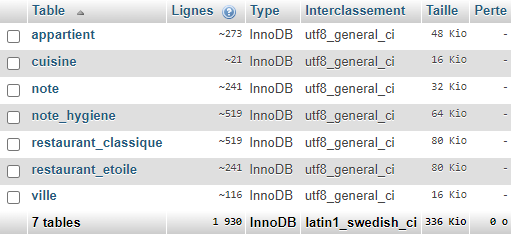
\includegraphics[width=10cm,height=5cm]{base.png}
\caption{Structure de la base de données.}\label{base}
}
\end{figure}

\hypertarget{moduxe9lisation-des-donnuxe9es}{%
\chapter{Modélisation des
Données}\label{moduxe9lisation-des-donnuxe9es}}

\hypertarget{moduxe9lisation-conceptuelle}{%
\section{Modélisation conceptuelle}\label{moduxe9lisation-conceptuelle}}

Avec nos jeux de données, nous avons construit un Modèle Conceptuel des
Données (MCD) avec l'outil en ligne mocodo utilisé lors des Tds comme
représenté sur la Figure \(~\)\ref{mcd} ci-dessous:

\begin{figure}
\hypertarget{mcd}{%
\centering
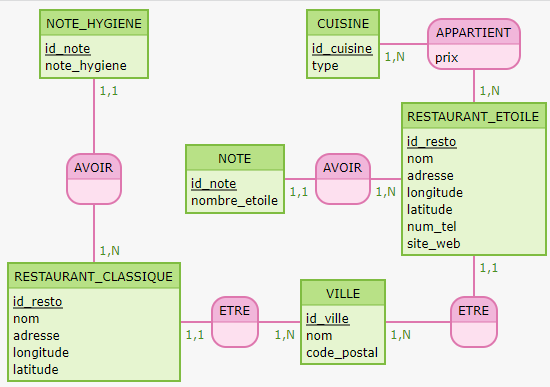
\includegraphics[width=10cm,height=5cm]{MCD.png}
\caption{Modèle Conceptuel des données.}\label{mcd}
}
\end{figure}

\bigskip

\hypertarget{moduxe9lisation-organisationnelle}{%
\section{Modélisation
organisationnelle}\label{moduxe9lisation-organisationnelle}}

A partir de ce modèle conceptuel, nous avons créé la version manuscrite
de notre Modèle Organisationnel de Données (MOD) :

RESTAURANT\_CLASSIQUE(id-resto, nom, adresse, longitude, latitude,
id\_ville) RESTAURANT\_ETOILE (id-resto-etoile, nom, adresse, longitude,
latitude, téléphone, id\_ville) VILLE (id\_ville, nom, code postal)
CUISINE (id-cuisine, type\_cuisine) NOTE (id-note, nombre\_etoiles,
id\_resto) NOTE\_HYGIENE(id-note, note\_hygiene, id\_resto) APPARTIENT
(id-resto-etoile, id-cuisine, prix)

\medskip

Nous avons ensuite créé ce modèle organisationnel sur notre base de
données grâce à l'outil Concepteur de WAMP - PhpMyAdmin afin de mieux
visualiser les liens entre les tables (clés étrangères) comme on peut le
voir sur la Figure \(~\)\ref{mod} ci-dessous:

\begin{figure}
\hypertarget{mod}{%
\centering
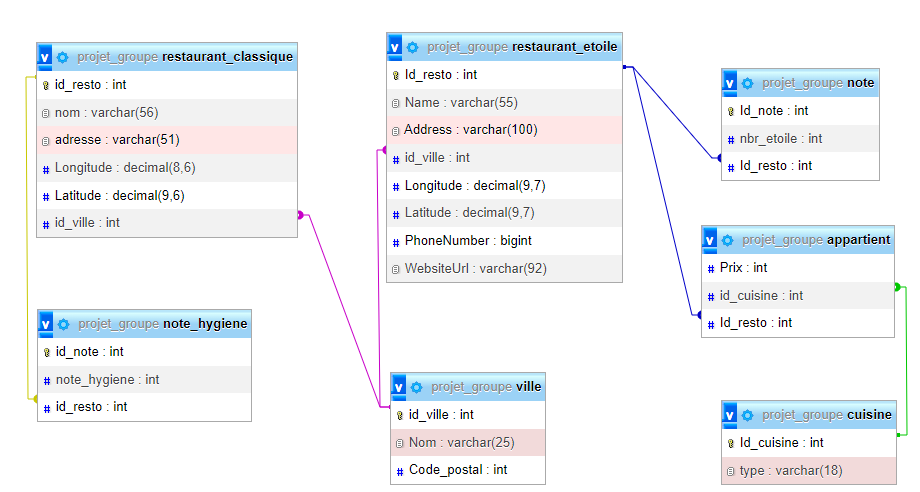
\includegraphics[width=10cm,height=5cm]{MOD.png}
\caption{Modèle Organisationnel des données.}\label{mod}
}
\end{figure}

\bigskip

\hypertarget{pruxe9traitement}{%
\chapter{Prétraitement}\label{pruxe9traitement}}

Afin d'importer nos données dans notre base, nous avons séparé les
tables dans des fichiers csv différents, en faisant correspondre les
données entre elles grâce à nos clés primaires et clés étrangères. Pour
ces dernières, nous avons dû ajouter des colonnes dans les tables afin
de pouvoir créer nos clés étrangères dans la base de données et donc les
liens entre les tables.

\medskip

Avant de réaliser l'import des données, nous avons remarqué que notre
table restaurant était trop volumineuse, nous avons donc dû supprimer
des données. Pour cela, nous avons gardé les restaurants dont les villes
étaient en commun avec les villes des restaurants étoilés. Nous sommes
donc passé de 11 658 lignes à 520 lignes.

\medskip

Après l'import dans SQL, nous avons modifié le type de certaines de nos
variables afin qu'elles aient le bon type et nous avons ensuite créé les
clés primaires et étrangères qui nous ont permis de générer le MOD situé
plus haut.

\hypertarget{requuxeates-en-sql-et-en-langage-naturel}{%
\chapter{Requêtes en SQL et en langage
naturel}\label{requuxeates-en-sql-et-en-langage-naturel}}

Afin de pouvoir répondre à notre problématique, nous avons effectué
plusieurs requêtes :

\begin{itemize}
\tightlist
\item
  \textbf{Restaurants étoilés qui ne sont pas à Paris (162 résultats)} :
\end{itemize}

\begin{Shaded}
\begin{Highlighting}[]
\NormalTok{SELECT restaurant\_etoile.Name, ville.Nom}
\NormalTok{FROM restaurant\_etoile, ville}
\NormalTok{WHERE ville.id\_ville}\OtherTok{=}\NormalTok{restaurant\_etoile.id\_ville}
\NormalTok{AND ville.Nom}\SpecialCharTok{!=}\StringTok{"Paris"}
\end{Highlighting}
\end{Shaded}

\medskip

\begin{itemize}
\tightlist
\item
  \textbf{Moyenne des notes hygiène par ville (39 résultats)} :
\end{itemize}

\begin{Shaded}
\begin{Highlighting}[]
\NormalTok{SELECT }\FunctionTok{AVG}\NormalTok{(note\_hygiene.note\_hygiene), ville.Nom }
\NormalTok{FROM note\_hygiene, restaurant\_classique, ville }
\NormalTok{WHERE ville.id\_ville}\OtherTok{=}\NormalTok{restaurant\_classique.id\_ville}
\NormalTok{AND note\_hygiene.id\_resto}\OtherTok{=}\NormalTok{restaurant\_classique.id\_resto}
\NormalTok{GROUP BY ville.id\_ville}
\NormalTok{HAVING }\FunctionTok{COUNT}\NormalTok{(restaurant\_classique.nom)}\SpecialCharTok{\textgreater{}}\DecValTok{1}
\end{Highlighting}
\end{Shaded}

\medskip

\begin{itemize}
\tightlist
\item
  \textbf{Le nom et la note moyenne de tous les restaurant étoilés (241
  résultats)} :
\end{itemize}

\begin{Shaded}
\begin{Highlighting}[]
\NormalTok{SELECT R.Name, }\FunctionTok{AVG}\NormalTok{(N.nbr\_etoile) AS }\StringTok{"note\_moyenne"}
\NormalTok{FROM restaurant\_etoile AS R}
\NormalTok{LEFT JOIN note AS N ON R.Id\_resto }\OtherTok{=}\NormalTok{ N.Id\_resto}
\NormalTok{GROUP BY R.Id\_resto}
\end{Highlighting}
\end{Shaded}

\medskip

\begin{itemize}
\tightlist
\item
  \textbf{Affiche les restaurants étoilés de 3 étoiles ainsi que les
  restaurants classiques ayant une note hygiène de 3 (149 résultats)} :
\end{itemize}

\begin{Shaded}
\begin{Highlighting}[]
\NormalTok{SELECT restaurant\_etoile.Name}
\NormalTok{FROM restaurant\_etoile, note}
\NormalTok{WHERE restaurant\_etoile.Id\_resto}\OtherTok{=}\NormalTok{note.Id\_resto}
\NormalTok{AND note.nbr\_etoile}\OtherTok{=}\DecValTok{3}
\NormalTok{UNION}
\NormalTok{SELECT restaurant\_classique.nom}
\NormalTok{FROM restaurant\_classique, note\_hygiene}
\NormalTok{WHERE restaurant\_classique.id\_resto}\OtherTok{=}\NormalTok{note\_hygiene.id\_resto}
\NormalTok{AND note\_hygiene.note\_hygiene}\OtherTok{=}\DecValTok{3}
\end{Highlighting}
\end{Shaded}

\medskip

\begin{itemize}
\tightlist
\item
  \textbf{Nombre d'étoile par ville, rangé par ordre décroissant (21
  résultats)} :
\end{itemize}

\begin{Shaded}
\begin{Highlighting}[]
\NormalTok{SELECT }\FunctionTok{sum}\NormalTok{(note.nbr\_etoile) as }\StringTok{"total etoiles par ville"}\NormalTok{, ville.Nom}
\NormalTok{FROM note, restaurant\_etoile, ville}
\NormalTok{WHERE ville.id\_ville}\OtherTok{=}\NormalTok{restaurant\_etoile.id\_ville}
\NormalTok{AND note.id\_resto}\OtherTok{=}\NormalTok{restaurant\_etoile.id\_resto}
\NormalTok{GROUP BY ville.id\_ville}
\NormalTok{HAVING }\FunctionTok{COUNT}\NormalTok{(restaurant\_etoile.name)}\SpecialCharTok{\textgreater{}}\DecValTok{1}
\NormalTok{order by }\FunctionTok{sum}\NormalTok{(note.nbr\_etoile) DESC }
\end{Highlighting}
\end{Shaded}

\hypertarget{moduxe9lisation-statistique-et-analyses}{%
\chapter{Modélisation statistique et
analyses}\label{moduxe9lisation-statistique-et-analyses}}

Diagramme des notes d'hygiènes par villes, Figure \(~\)\ref{diag1} :

\begin{figure}
\hypertarget{diag1}{%
\centering
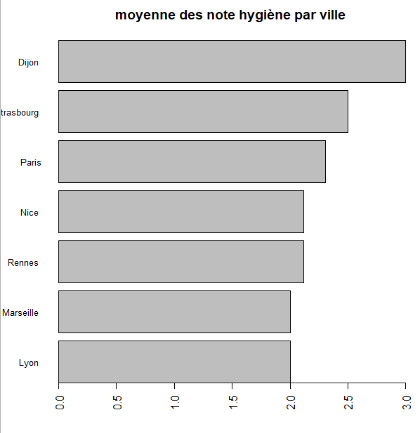
\includegraphics[width=10cm,height=15cm]{diag_moy_note_hyg.png}
\caption{Première modélisation}\label{diag1}
}
\end{figure}

\bigskip
\bigskip

Ce graphique en barre permet de comparer les notes d'hygiène entre sept
villes de France : Paris, Marseille, Dijon, Lyon, Nice, Rennes et
Strasbourg qui sont affichées sur l'axe des y, Les notes d'hygiène sont
évaluées de 1 à 3 et présentées sur l'axe des x. Le graphique montre que
la ville de Dijon à la note d'hygiène la plus élevée suivie de
Strasbourg et Paris. Nice et Rennes ont la même note d'hygiène. Tandis
que Marseille et Lyon ont les notes d'hygiène les plus basses. Cette
analyse indique que la moyenne des notes hygiènes varient entre les
villes, et que certaines villes obtiennent de meilleurs résultats que
d'autres en termes de qualité d'hygiène dans les restaurants. Ces
résultats peuvent être utilisés pour identifier les villes qui ont
besoin d'améliorer leurs pratiques d'hygiène et pour encourager les
restaurants à respecter des normes élevées en matière d'hygiène
alimentaire. \bigskip

Diagramme du nombre de restaurants étoilés par ville, Figure
\(~\)\ref{diag2} :

\begin{figure}
\hypertarget{diag2}{%
\centering
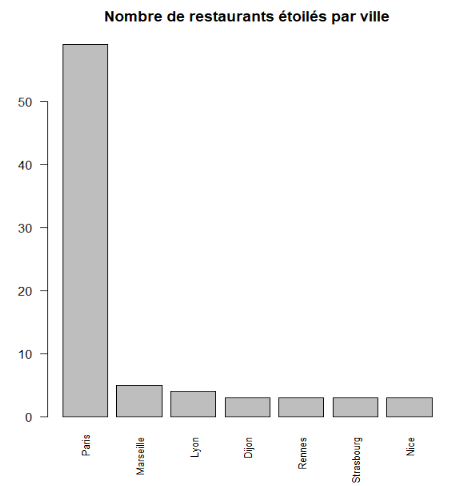
\includegraphics[width=13cm,height=15cm]{diag_nb_resto_etoile.png}
\caption{Deuxième modélisation}\label{diag2}
}
\end{figure}

\bigskip
\bigskip

Ce graphique montre le nombre de restaurants étoilés dans les sept
villes françaises. Le nombre de restaurants est affiché sur l'axe des y,
tandis que les villes sont indiquées sur l'axe des x. On observe que
Paris est la ville qui possède le plus grand nombre de restaurants
étoilés. Marseille arrive en deuxième position suivie de Lyon et Dijon.
Les villes restantes (Rennes, Strasbourg, Nice) ont un nombre de
restaurants bien inférieur et presque équivalent. Il est important de
noter que ces données ne prennent en compte que les restaurants qui ont
reçu au moins une étoile. Les restaurants qui n'ont pas d'étoile ne sont
pas pris en compte dans ce graphique. En conclusion, ce graphique montre
clairement que Paris est la ville française qui possède le plus grand
nombre de restaurants étoilés. Marseille et Lyon sont également des
villes importantes pour la gastronomie française mais leur nombre de
restaurants étoilés est bien inférieur à celui de Paris.

\bigskip

Diagramme des prix moyens des restaurants étoilés par villes, Figure
\(~\)\ref{diag3}:

\begin{figure}
\hypertarget{diag3}{%
\centering
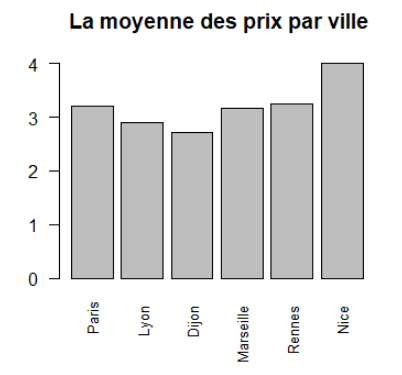
\includegraphics[width=10cm,height=15cm]{diag_moy_prix.png}
\caption{Troisième modélisation}\label{diag3}
}
\end{figure}

\bigskip

Le graphe représente la moyenne des prix de restaurants de six villes
différentes. Les barres représentent la moyenne des prix de chaque
ville, avec la plus haute barre indiquant la ville avec la moyenne des
prix la plus élevée. L'analyse des résultats montre que Nice a la
moyenne de prix la plus élevée, suivie de Rennes et Paris puis de
Marseille, Lyon et Dijon. Cela signifie que les restaurants de la ville
de Nice sont en moyenne plus chers que ceux des autres villes. Cette
information peut être utilisée pour diverses analyses. Par exemple, pour
une personne qui planifie un voyage gastronomique et qui a un budget
limité, il pourrait être judicieux de choisir une ville autre que Paris
ou Nice. Les villes ayant une moyenne de prix plus basse (Marseille,
Lyon et Dijon) pourraient être de bonnes options pour cette personne,
car elle pourrait profiter d'une expérience culinaire similaire à un
prix plus abordable. De même, pour les entreprises du secteur de la
restauration, les villes ayant une moyenne de prix plus basse pourraient
être plus avantageuse pour minimiser les coûts d'exploitation.

\bigskip

Carte de France représentant les villes ayant des restaurant étoilés,
Figure \(~\)\ref{diag5} :

\begin{figure}
\hypertarget{diag5}{%
\centering
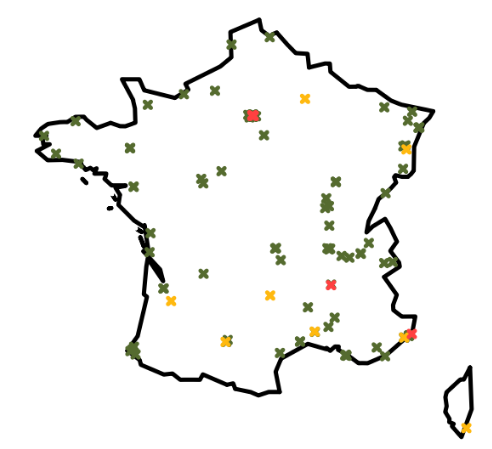
\includegraphics[width=10cm,height=13cm]{carte.png}
\caption{Cinquième modélisation}\label{diag5}
}
\end{figure}

\medskip

La carte montre la répartition spatiale des restaurants étoilés en
France, en distinguant ceux qui ont une étoile, deux étoiles, et trois
étoiles. Les points vert foncé représentent les restaurants avec une
étoile, les points jaunes representent ceux avec deux étoiles et les
points marrons représentent les restaurants avec trois étoiles. On peut
observer que les restaurants étoilés sont concentrés dans certaines
régions notamment en Île-de-France, dans le Sud-Est de la France et dans
la région de la Nouvelle Aquitaine. On observe également que Paris est
la ville avec le plus grand nombre de restaurants étoilés en France,
avec une concentration élevée de restaurants avec trois étoiles. En
revanche, d'autres régions de la France semblent moins bien représentées
en termes de restaurants étoilés, comme la région du Grand-Est ou de la
Normandie. Cela pourrait être dû à des facteurs tels que le manque de
tradition gastronomique dans ces régions ou à une concurrence plus forte
pour des restaurants gastronomiques dans les régions moins touristiques.
On peut également noter que la densité de restaurants étoilés diminue à
mesure que l'on s'éloigne des grandes villes ou des régions les plus
touristiques. Enfin, la différence de densité entre les restaurants
étoilés avec une, deux, ou trois étoiles peut être expliquée par la
difficulté croissante d'obtenir une étoile supplémentaire, ce qui peut
limiter le nombre de restaurants étoilés avec deux ou trois étoiles par
rapport aux restaurants étoilés avec une étoile.

\bigskip

\hypertarget{conclusion-et-perspectives}{%
\chapter{Conclusion et perspectives}\label{conclusion-et-perspectives}}

Après avoir étudié et analysé les graphiques des parties ``Modélisations
statistiques et analyses'' et ``Annexes'', on peut conclure que les
grandes villes où l'on mange le mieux en tenant compte uniquement des
restaurants étoilés et des notes d'hygiènes de restaurants non-étoilés,
sont Paris, en tête du classement, avec Marseille, Lyon et Nice à la
suite. En effet, ces trois dernières sont souvent classées dans le top
trois des différents graphiques.

\medskip

Cette conclusion ainsi que les analyses précédente sont valables dans le
cadre de notre problématique ciblée. En effet, le sujet ``Où mange-t-on
le mieux'' est vaste et peut-être interprété différemment selon les
besoins. Ainsi, d'autres jeux de données et modélisations seront plus
adaptés à d'autres besoins, par exemple si l'on se concentre sur le type
de restauration (restauration collective, restaurants de vile, etc.).

\bigskip

\textbf{Problèmes rencontrés:}

\hypertarget{annexes}{%
\chapter*{Annexes}\label{annexes}}
\addcontentsline{toc}{chapter}{Annexes}

\hypertarget{bibliographie}{%
\section*{Bibliographie}\label{bibliographie}}
\addcontentsline{toc}{section}{Bibliographie}

\hypertarget{refs}{}
\begin{CSLReferences}{0}{0}
\end{CSLReferences}

\bibliographystyle{elsarticle-harv}
\bibliography{references}

\bigskip

\hypertarget{diagramme-suppluxe9mentaire}{%
\section{\texorpdfstring{\textbf{Diagramme
supplémentaire}}{Diagramme supplémentaire}}\label{diagramme-suppluxe9mentaire}}

Diagramme du nombre d'étoiles par ville , Figure \(~\)\ref{diag4} :

\begin{figure}
\hypertarget{diag4}{%
\centering
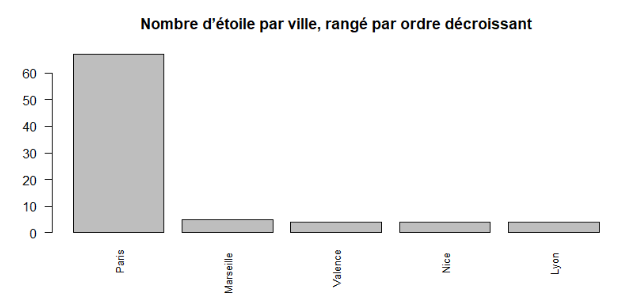
\includegraphics[width=15cm,height=10cm]{diag_nb_etoile_par_ville.png}
\caption{Quatrième modélisation}\label{diag4}
}
\end{figure}

\bigskip

Ce graphique représente le nombre d'étoiles attribuées aux restaurants
de chaque ville. Les cinq villes ayant le plus grand nombre d'étoiles
sont affichées sur le graphique, classées par ordre décroissant. On peut
voir que Paris a le plus grand nombre d'étoiles attribuées, suivi de
Marseille, Valence, Nice et Lyon qui ont toutes un nombre d'étoiles
assez similaire. Cela suggère que ces villes ont un grand nombre de
restaurants renommés, qui ont reçu des étoiles Michelin en récompense de
leur cuisine de haute qualité. En général, ce graphique peut être
utilisé pour aider à identifier les tendances en matière de gastronomie
et les centres de restauration renommés dans les différentes villes.

\hypertarget{codes}{%
\section*{\texorpdfstring{\textbf{Codes}}{Codes}}\label{codes}}
\addcontentsline{toc}{section}{\textbf{Codes}}

Code de la carte de France (Figure 6.5) : \tiny

\begin{Shaded}
\begin{Highlighting}[]
\FunctionTok{install.packages}\NormalTok{(}\StringTok{"RMySQL"}\NormalTok{)}

\FunctionTok{install.packages}\NormalTok{(}\StringTok{"DBI"}\NormalTok{)}
\FunctionTok{library}\NormalTok{(DBI)}

\NormalTok{bd }\OtherTok{\textless{}{-}}\NormalTok{ DBI}\SpecialCharTok{::}\FunctionTok{dbConnect}\NormalTok{(RMySQL}\SpecialCharTok{::}\FunctionTok{MySQL}\NormalTok{(),}
                     
                     \AttributeTok{host =} \StringTok{"9ha.h.filess.io"}\NormalTok{, }\AttributeTok{port =} \DecValTok{3307}\NormalTok{,}
                     \AttributeTok{username =} \StringTok{"ProjetBD\_believedbe"}\NormalTok{, }
                     \AttributeTok{password =} \StringTok{"83c50259163a65e8ca715f92e1bbb9c15d0ca7a9"}\NormalTok{, }
                     \AttributeTok{dbname =} \StringTok{"ProjetBD\_believedbe"}\NormalTok{)}

\FunctionTok{dbListTables}\NormalTok{(bd)}

\NormalTok{requete3 }\OtherTok{\textless{}{-}} \StringTok{"SELECT restaurant\_etoile.latitude, restaurant\_etoile.longitude     }
\StringTok{FROM restaurant\_etoile, note                }
\StringTok{where note.id\_resto=restaurant\_etoile.id\_resto}
\StringTok{and note.nbr\_etoile=3;}

\StringTok{"}
\NormalTok{requete2 }\OtherTok{\textless{}{-}} \StringTok{"SELECT restaurant\_etoile.latitude, restaurant\_etoile.longitude     }
\StringTok{FROM restaurant\_etoile, note                }
\StringTok{where note.id\_resto=restaurant\_etoile.id\_resto}
\StringTok{and note.nbr\_etoile=2;}
\StringTok{"}
\NormalTok{requete }\OtherTok{\textless{}{-}} \StringTok{"SELECT restaurant\_etoile.latitude, restaurant\_etoile.longitude      }
\StringTok{FROM restaurant\_etoile, note                }
\StringTok{where note.id\_resto=restaurant\_etoile.id\_resto}
\StringTok{and note.nbr\_etoile=1;}
\StringTok{"}
\NormalTok{resultatetoile3 }\OtherTok{\textless{}{-}} \FunctionTok{dbSendQuery}\NormalTok{(bd, requete3)}

\NormalTok{resetoile3}\OtherTok{\textless{}{-}}\FunctionTok{fetch}\NormalTok{(resultatetoile3)}

\NormalTok{resultatetoile2 }\OtherTok{\textless{}{-}} \FunctionTok{dbSendQuery}\NormalTok{(bd, requete2)}

\NormalTok{resetoile2}\OtherTok{\textless{}{-}}\FunctionTok{fetch}\NormalTok{(resultatetoile2)}

\NormalTok{resultatetoile }\OtherTok{\textless{}{-}} \FunctionTok{dbSendQuery}\NormalTok{(bd, requete)}

\NormalTok{resetoile}\OtherTok{\textless{}{-}}\FunctionTok{fetch}\NormalTok{(resultatetoile)}

\FunctionTok{dbDisconnect}\NormalTok{(bd)}

\FunctionTok{install.packages}\NormalTok{(}\StringTok{"maps"}\NormalTok{)}
\FunctionTok{install.packages}\NormalTok{(}\StringTok{"mapdata"}\NormalTok{)}

\FunctionTok{library}\NormalTok{(maps)}
\FunctionTok{library}\NormalTok{(mapdata)}
\FunctionTok{map}\NormalTok{(}\StringTok{"worldHires"}\NormalTok{, }\StringTok{"france"}\NormalTok{, }\AttributeTok{xlim=}\FunctionTok{c}\NormalTok{(}\SpecialCharTok{{-}}\DecValTok{5}\NormalTok{,}\DecValTok{10}\NormalTok{), }\AttributeTok{ylim=}\FunctionTok{c}\NormalTok{(}\DecValTok{35}\NormalTok{,}\DecValTok{55}\NormalTok{))}
\NormalTok{etoile1lat}\OtherTok{\textless{}{-}}\FunctionTok{subset}\NormalTok{(resetoile, }\AttributeTok{select =}\NormalTok{ latitude)}
\NormalTok{etoile1long}\OtherTok{\textless{}{-}}\FunctionTok{subset}\NormalTok{(resetoile, }\AttributeTok{select =}\NormalTok{ longitude)}
\NormalTok{etoile2lat}\OtherTok{\textless{}{-}}\FunctionTok{subset}\NormalTok{(resetoile2, }\AttributeTok{select =}\NormalTok{ latitude)}
\NormalTok{etoile2long}\OtherTok{\textless{}{-}}\FunctionTok{subset}\NormalTok{(resetoile2, }\AttributeTok{select =}\NormalTok{ longitude)}
\NormalTok{etoile3lat}\OtherTok{\textless{}{-}}\FunctionTok{subset}\NormalTok{(resetoile3, }\AttributeTok{select =}\NormalTok{ latitude)}
\NormalTok{etoile3long}\OtherTok{\textless{}{-}}\FunctionTok{subset}\NormalTok{(resetoile3, }\AttributeTok{select =}\NormalTok{ longitude)}

\FunctionTok{points}\NormalTok{(}\FunctionTok{unlist}\NormalTok{(etoile1long),}\FunctionTok{unlist}\NormalTok{(etoile1lat),}\AttributeTok{pch=}\DecValTok{4}\NormalTok{,}\AttributeTok{cex=}\FloatTok{0.2}\NormalTok{, }\AttributeTok{col=}\StringTok{"darkolivegreen"}\NormalTok{)}
\FunctionTok{points}\NormalTok{(}\FunctionTok{unlist}\NormalTok{(etoile2long), }\FunctionTok{unlist}\NormalTok{(etoile2lat), }\AttributeTok{pch=}\DecValTok{4}\NormalTok{, }\AttributeTok{cex=}\FloatTok{0.2}\NormalTok{, }\AttributeTok{col=}\StringTok{"darkgoldenrod1"}\NormalTok{)}
\FunctionTok{points}\NormalTok{(}\FunctionTok{unlist}\NormalTok{(etoile3long),}\FunctionTok{unlist}\NormalTok{(etoile3lat),}\AttributeTok{pch=}\DecValTok{4}\NormalTok{,}\AttributeTok{cex=}\FloatTok{0.2}\NormalTok{,}\AttributeTok{col=}\StringTok{"brown1"}\NormalTok{)}
\end{Highlighting}
\end{Shaded}

\normalsize
\bigskip

Code du graphique moyenne des notes hygiènes par ville (Figure 6.1):
\tiny

\begin{Shaded}
\begin{Highlighting}[]
\FunctionTok{install.packages}\NormalTok{(}\StringTok{"RMySQL"}\NormalTok{)}
\FunctionTok{install.packages}\NormalTok{(}\StringTok{"DBI"}\NormalTok{)}

\FunctionTok{ldbDisconnect}\NormalTok{(bd)}
\FunctionTok{library}\NormalTok{(DBI)}
\NormalTok{bd }\OtherTok{\textless{}{-}}\NormalTok{ DBI}\SpecialCharTok{::}\FunctionTok{dbConnect}\NormalTok{(RMySQL}\SpecialCharTok{::}\FunctionTok{MySQL}\NormalTok{(),}
                     
                     \AttributeTok{host =} \StringTok{"9ha.h.filess.io"}\NormalTok{, }\AttributeTok{port =} \DecValTok{3307}\NormalTok{,}
                     \AttributeTok{username =} \StringTok{"ProjetBD\_believedbe"}\NormalTok{,}
                     \AttributeTok{password =} \StringTok{"83c50259163a65e8ca715f92e1bbb9c15d0ca7a9"}\NormalTok{,}
                     \AttributeTok{dbname =} \StringTok{"ProjetBD\_believedbe"}\NormalTok{)}

\FunctionTok{dbListTables}\NormalTok{(bd)}

\NormalTok{requete }\OtherTok{\textless{}{-}}\StringTok{"SELECT AVG(note\_hygiene.note\_hygiene), ville.Nom }
\StringTok{  FROM note\_hygiene, restaurant\_classique, ville                }
\StringTok{  WHERE ville.id\_ville=restaurant\_classique.id\_ville}
\StringTok{  AND note\_hygiene.id\_resto=restaurant\_classique.id\_resto}
\StringTok{  AND ville.Nom in (\textquotesingle{}Paris\textquotesingle{},\textquotesingle{}Marseille\textquotesingle{},\textquotesingle{}dijon\textquotesingle{},\textquotesingle{}Lyon\textquotesingle{},\textquotesingle{}Nice\textquotesingle{},\textquotesingle{}Rennes\textquotesingle{},’Strasbourg’)}
\StringTok{  GROUP BY ville.Nom}
\StringTok{  ORDER BY AVG(note\_hygiene.note\_hygiene) ASC}
\StringTok{"}

\NormalTok{resultatetoile }\OtherTok{\textless{}{-}} \FunctionTok{dbSendQuery}\NormalTok{(bd, requete)}

\NormalTok{resetoile}\OtherTok{\textless{}{-}}\FunctionTok{fetch}\NormalTok{(resultatetoile)}

\FunctionTok{attach}\NormalTok{(resetoile)}
\FunctionTok{head}\NormalTok{(resetoile)}

\FunctionTok{barplot}\NormalTok{(}\StringTok{\textasciigrave{}}\AttributeTok{AVG(note\_hygiene.note\_hygiene)}\StringTok{\textasciigrave{}}\NormalTok{,}\AttributeTok{names.arg =}\NormalTok{ Nom, }\AttributeTok{las=} \DecValTok{2}\NormalTok{, }\AttributeTok{horiz=} \ConstantTok{TRUE}\NormalTok{, }\AttributeTok{cex.names =} \FloatTok{0.8}\NormalTok{)}
\FunctionTok{title}\NormalTok{(}\StringTok{"moyenne des note hygiène par ville"}\NormalTok{)}
\end{Highlighting}
\end{Shaded}

\normalsize
\bigskip

Code du graphique nombre de restaurants étoilés par ville (Figure 6.2) :
\tiny

\begin{Shaded}
\begin{Highlighting}[]
\FunctionTok{dbDisconnect}\NormalTok{(bd)}
\FunctionTok{library}\NormalTok{(DBI)}
\NormalTok{bd }\OtherTok{\textless{}{-}}\NormalTok{ DBI}\SpecialCharTok{::}\FunctionTok{dbConnect}\NormalTok{(RMySQL}\SpecialCharTok{::}\FunctionTok{MySQL}\NormalTok{(),}
                     
                     \AttributeTok{host =} \StringTok{"9ha.h.filess.io"}\NormalTok{, }\AttributeTok{port =} \DecValTok{3307}\NormalTok{,}
                     \AttributeTok{username =} \StringTok{"ProjetBD\_believedbe"}\NormalTok{,}
                     \AttributeTok{password =} \StringTok{"83c50259163a65e8ca715f92e1bbb9c15d0ca7a9"}\NormalTok{,}
                     \AttributeTok{dbname =} \StringTok{"ProjetBD\_believedbe"}\NormalTok{)}

\FunctionTok{dbListTables}\NormalTok{(bd)}

\NormalTok{requete3 }\OtherTok{\textless{}{-}}\StringTok{"SELECT COUNT(restaurant\_etoile.id\_resto), ville.Nom     }
\StringTok{FROM note, ville, restaurant\_etoile             }
\StringTok{WHERE ville.id\_ville=restaurant\_etoile.id\_ville}
\StringTok{AND note.id\_resto=restaurant\_etoile.id\_resto}
\StringTok{and note.nbr\_etoile\textgreater{}0}
\StringTok{GROUP BY ville.id\_ville}
\StringTok{order by COUNT(restaurant\_etoile.id\_resto) desc}
\StringTok{limit 7}
\StringTok{"}

\NormalTok{resultatetoile3 }\OtherTok{\textless{}{-}} \FunctionTok{dbSendQuery}\NormalTok{(bd, requete3)}

\NormalTok{resetoile3}\OtherTok{\textless{}{-}}\FunctionTok{fetch}\NormalTok{(resultatetoile3)}

\FunctionTok{attach}\NormalTok{(resetoile3)}
\FunctionTok{head}\NormalTok{(resetoile3)}

\FunctionTok{barplot}\NormalTok{(}\StringTok{\textasciigrave{}}\AttributeTok{COUNT(restaurant\_etoile.id\_resto)}\StringTok{\textasciigrave{}}\NormalTok{,}\AttributeTok{names.arg =}\NormalTok{ Nom, }\AttributeTok{cex.names =} \FloatTok{0.8}\NormalTok{, }\AttributeTok{las=}\DecValTok{2}\NormalTok{)}
\FunctionTok{title}\NormalTok{(}\StringTok{"Nombre de restaurants étoilés par ville"}\NormalTok{)}
\end{Highlighting}
\end{Shaded}

\normalsize
\bigskip

Code du graphique moyenne des prix des restaurants étoilés par ville
(Figure 6.3) : \tiny

\begin{Shaded}
\begin{Highlighting}[]
\FunctionTok{dbDisconnect}\NormalTok{(bd)}
\FunctionTok{library}\NormalTok{(DBI)}
\NormalTok{bd }\OtherTok{\textless{}{-}}\NormalTok{ DBI}\SpecialCharTok{::}\FunctionTok{dbConnect}\NormalTok{(RMySQL}\SpecialCharTok{::}\FunctionTok{MySQL}\NormalTok{(),}
                     
                     \AttributeTok{host =} \StringTok{"9ha.h.filess.io"}\NormalTok{, }\AttributeTok{port =} \DecValTok{3307}\NormalTok{,}
                     \AttributeTok{username =} \StringTok{"ProjetBD\_believedbe"}\NormalTok{,}
                     \AttributeTok{password =} \StringTok{"83c50259163a65e8ca715f92e1bbb9c15d0ca7a9"}\NormalTok{,}
                     \AttributeTok{dbname =} \StringTok{"ProjetBD\_believedbe"}\NormalTok{)}

\FunctionTok{dbListTables}\NormalTok{(bd)}

\NormalTok{requete4 }\OtherTok{\textless{}{-}}\StringTok{"SELECT V.Nom, avg(A.Prix) prix\_moyen}
\StringTok{FROM restaurant\_etoile R, ville V, appartient A, note}
\StringTok{WHERE A.Id\_resto=R.Id\_resto}
\StringTok{and V.Nom in (\textquotesingle{}Paris\textquotesingle{},\textquotesingle{}Marseille\textquotesingle{},\textquotesingle{}dijon\textquotesingle{},\textquotesingle{}Lyon\textquotesingle{},\textquotesingle{}Nice\textquotesingle{},\textquotesingle{}Rennes\textquotesingle{})}
\StringTok{AND R.id\_ville=V.id\_ville}
\StringTok{and note.id\_resto=R.id\_resto}
\StringTok{GROUP BY V.Nom}
\StringTok{ORDER BY count(R.id\_resto) desc}


\StringTok{"}

\NormalTok{resultatetoile4 }\OtherTok{\textless{}{-}} \FunctionTok{dbSendQuery}\NormalTok{(bd, requete4)}

\NormalTok{resetoile4}\OtherTok{\textless{}{-}}\FunctionTok{fetch}\NormalTok{(resultatetoile4)}

\FunctionTok{attach}\NormalTok{(resetoile4)}
\FunctionTok{head}\NormalTok{(resetoile4)}

\FunctionTok{barplot}\NormalTok{(}\StringTok{\textasciigrave{}}\AttributeTok{prix\_moyen}\StringTok{\textasciigrave{}}\NormalTok{, }\AttributeTok{names.arg =}\NormalTok{ Nom, }\AttributeTok{cex.names =} \FloatTok{0.8}\NormalTok{, }\AttributeTok{las=}\DecValTok{2}\NormalTok{)}
\FunctionTok{title}\NormalTok{(}\StringTok{" La moyenne des prix par ville"}\NormalTok{)}
\end{Highlighting}
\end{Shaded}

\normalsize
\bigskip

Code du graphique du nombre d'étoile par ville rangé par ordre
décroissant (Figure 6.4) : \tiny

\begin{Shaded}
\begin{Highlighting}[]
\FunctionTok{library}\NormalTok{(DBI)}
\NormalTok{bd }\OtherTok{\textless{}{-}}\NormalTok{ DBI}\SpecialCharTok{::}\FunctionTok{dbConnect}\NormalTok{(RMySQL}\SpecialCharTok{::}\FunctionTok{MySQL}\NormalTok{(),}
                     
                     \AttributeTok{host =} \StringTok{"9ha.h.filess.io"}\NormalTok{, }\AttributeTok{port =} \DecValTok{3307}\NormalTok{,}
                     \AttributeTok{username =} \StringTok{"ProjetBD\_believedbe"}\NormalTok{,}
                     \AttributeTok{password =} \StringTok{"83c50259163a65e8ca715f92e1bbb9c15d0ca7a9"}\NormalTok{,}
                     \AttributeTok{dbname =} \StringTok{"ProjetBD\_believedbe"}\NormalTok{)}

\FunctionTok{dbListTables}\NormalTok{(bd)}

\NormalTok{requete2 }\OtherTok{\textless{}{-}}\StringTok{"SELECT sum(note.nbr\_etoile), ville.Nom}
\StringTok{ FROM note, restaurant\_etoile, ville}
\StringTok{ WHERE ville.id\_ville=restaurant\_etoile.id\_ville}
\StringTok{ AND note.id\_resto=restaurant\_etoile.id\_resto}
\StringTok{ GROUP BY ville.id\_ville}
\StringTok{ HAVING COUNT(restaurant\_etoile.name)\textgreater{}1}
\StringTok{ order by sum(note.nbr\_etoile) desc}
\StringTok{ limit 5}
\StringTok{"}

\NormalTok{resultatetoile2 }\OtherTok{\textless{}{-}} \FunctionTok{dbSendQuery}\NormalTok{(bd, requete2)}

\NormalTok{resetoile2}\OtherTok{\textless{}{-}}\FunctionTok{fetch}\NormalTok{(resultatetoile2)}

\FunctionTok{attach}\NormalTok{(resetoile2)}

\FunctionTok{head}\NormalTok{(resetoile2)}

\FunctionTok{barplot}\NormalTok{(}\StringTok{\textasciigrave{}}\AttributeTok{sum(note.nbr\_etoile)}\StringTok{\textasciigrave{}}\NormalTok{, }\AttributeTok{names.arg =}\NormalTok{ Nom,}\AttributeTok{las=} \DecValTok{2}\NormalTok{,}\AttributeTok{cex.names =} \FloatTok{0.8}\NormalTok{)}
\FunctionTok{title}\NormalTok{(}\StringTok{"Nombre d’étoile par ville, rangé par ordre décroissant"}\NormalTok{)}
\end{Highlighting}
\end{Shaded}

\normalsize







\end{document}

